\part{Exceptions}
\frame{\partpage}

\begin{frame}{Exceptions}
	\begin{itemize}
		\pause\item You've all seen them already...
	\end{itemize}
	\begin{center}
		\pause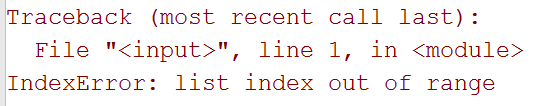
\includegraphics[width=0.5\textwidth]{exception}
	\end{center}
	\begin{itemize}
		\pause\item Some operations in a program can fail
		\pause\item Exceptions are a way of signalling that failure
	\end{itemize}
\end{frame}

\begin{frame}[fragile]{Raising exceptions}
	\pause
	\begin{lstlisting}
def factorial(n):
    if n < 0:
        raise ValueError("Argument must be positive")
	\end{lstlisting}
	\begin{itemize}
		\pause\item \lstinline{ValueError} is a built-in class
		\pause\item Its initialiser takes one argument: a human-readable
			string describing the error
		\pause\item The exception is an \textbf{instance} of the
			\lstinline{ValueError} class
	\end{itemize}
\end{frame}

\begin{frame}{Built-in exception types}
	\footnotesize\url{https://docs.python.org/2/library/exceptions.html}
\end{frame}

\begin{frame}[fragile]{Custom exception types}
	\pause
	\begin{lstlisting}
class UnreticulatedSplineError(Exception):
    def __init__(self, message):
		    Exception.__init__(self, message)

...
if not spline.is_reticulated():
    raise UnreticulatedSplineError("Spline must be reticulated")
	\end{lstlisting}
	\begin{itemize}
		\pause\item Inherit from built-in class \lstinline{Exception}
		\pause\item Just like any other class --- can contain any required
			fields and methods
	\end{itemize}
\end{frame}

\begin{frame}[fragile]{Catching exceptions}
	\begin{lstlisting}
try:
    input_file = open(filename, "rt")
except IOError:
    print "Failed to open file, please select a different one"
	\end{lstlisting}
	\begin{itemize}
		\pause\item If anything inside the \lstinline{try} block throws an
			\lstinline{IOError} (or a subclass of \lstinline{IOError}),
			the \lstinline{except} block executes
		\pause\item A \lstinline{try} block can have several \lstinline{except}
			blocks for different exception types
		\pause\item An uncaught exception kills the program
	\end{itemize}
\end{frame}

\begin{frame}{Exceptions and control flow}
	\begin{itemize}
		\pause\item Raising exception transfers control to the innermost matching
			\lstinline{except} handler
		\pause\item This can result in breaking out of loops and functions
		\pause\item This can be powerful in the hands of a good programmer...
		\pause\item ... or confusing in the hands of a bad one
	\end{itemize}
\end{frame}

\begin{frame}{Types of exceptions}
	There are two types of exceptions...
	\begin{itemize}
		\pause\item Those intended to catch \textbf{runtime errors}
			(e.g.\ missing files, insufficient resources, invalid input, ...)
			\begin{itemize}
				\pause\item Good software should \textbf{catch} and \textbf{recover} from these
			\end{itemize}
		\pause\item Those intended to catch \textbf{programmer errors}
			(e.g.\ type mismatch, index out of bounds, divide by zero, ...)
			\begin{itemize}
				\pause\item Generally best to let these crash the program so that the programmer can notice and fix them
				\pause\item A commercially released program might catch them to allow the user to submit a bug report to the developer
			\end{itemize}
	\end{itemize}
\end{frame}

\begin{frame}[fragile]{Assertions}
	\begin{itemize}
		\pause\item \lstinline{AssertionError} is a special exception type for catching programmer errors
		\pause\item Can be raised with the following syntax:
	\end{itemize}
	\begin{lstlisting}
assert n > 0, "n must be positive"
	\end{lstlisting}
	\begin{itemize}
		\pause\item The exception is raised if the condition is \lstinline{False}
		\pause\item \lstinline{assert} should \textbf{only} be used to catch programmer errors,
			therefore you should \textbf{never} try to handle \lstinline{AssertionError} in a \lstinline{try ... except}
			block
		\pause\item In some programming languages, assertions are stripped out of ``Release'' builds ---
			so avoid assertions with side-effects!
	\end{itemize}
\end{frame}

\begin{frame}[fragile]{More options with try blocks}
	\begin{lstlisting}
try:
    input_file = open(filename, "rt")
except IOError as err:
    print "File error:", err
else:
    print "This only executes if the try block did not raise an exception"
finally:
    print "This executes whether or not the try block raised an exception, even if there were uncaught exceptions"
	\end{lstlisting}
\end{frame}

\begin{frame}[fragile]{It's easier to ask forgiveness than permission}
	\pause I.e.\ it's better to catch exceptions
		than to use \lstinline{if} statements to avoid them
	\pause\begin{lstlisting}
try:
    x = list[index]
except IndexError:
    x = None
	\end{lstlisting}
	This is ``more Pythonic'' than this:
	\pause\begin{lstlisting}
if index >= 0 and index < len(list):
    x = list[index]
else:
    x = None
	\end{lstlisting}
\end{frame}
